\documentclass[a4paper,12pt]{article}
\usepackage[utf8]{inputenc}
\usepackage[ngerman]{babel}
\usepackage{amsmath}
\usepackage{amssymb}
\usepackage{amsthm}
\usepackage{geometry}
\usepackage{graphicx}
\usepackage[hidelinks]{hyperref}
\usepackage{listings}
\usepackage{xcolor}
\usepackage{enumitem}
\usepackage{booktabs}
\usepackage{float}

\geometry{margin=2.5cm}

\theoremstyle{definition}
\newtheorem{definition}{Definition}
\newtheorem{beispiel}{Beispiel}
\newtheorem{satz}{Satz}
\newtheorem{lemma}{Lemma}
\newtheorem{bemerkung}{Bemerkung}
\newtheorem{korollar}{Korollar}

\setlist[itemize,1]{label=--}

\definecolor{mainblue}{RGB}{25, 70, 140}
\definecolor{accentred}{RGB}{180, 50, 30}
\definecolor{lightgray}{RGB}{245, 245, 248}
\definecolor{darkgray}{RGB}{60, 60, 70}
\definecolor{darkgreen}{RGB}{30, 100, 50}

\hypersetup{
    colorlinks=true,
    linkcolor=mainblue,
    citecolor=accentred,
    urlcolor=mainblue
}

\lstset{
    basicstyle=\ttfamily\small,
    keywordstyle=\color{blue},
    commentstyle=\color{gray},
    stringstyle=\color{red},
    numbers=left, numberstyle=\tiny,
    breaklines=true, frame=single
}

\title{\textbf{Explosive Konvektionsst\"{o}rung zur Pr\"{a}vention\\
tropischer Wirbelsturmsysteme}\\[0.6em]
\large Ein formales Modell der ballistischen Druckwellenintervention\\
in der Thermodynamischen Instabilit\"{a}tszone (TIZ)}
\author{Stephan Epp\\[0.3em]
\small Universit\"{a}t Bielefeld, Fakult\"{a}t f\"{u}r Informatik}
\date{25.\ Mai 2026}

\begin{document}

\maketitle

\begin{abstract}
Tropische Wirbelsturmsysteme (Hurrikane) entstehen durch ein komplexes Wechselspiel
thermodynamischer Instabilit\"{a}ten an der Grenzzone zwischen warmen und kalten
Luftmassen \"{u}ber tropischen Ozeanen.
Diese Arbeit entwickelt ein formales Modell der \emph{Explosiven Konvektionsst\"{o}rung}
(EKS): Ein \emph{Ballistisches Interventionssystem} (BIS) befF\"{o}rdert einen
Sprengk\"{o}rper pr\"{a}zise in die \emph{Thermodynamische Instabilit\"{a}tszone} (TIZ),
detoniert dort an der mathematisch optimalen Position $x^{*}$ und erzeugt einen
impulsiven Druckgradienten, der die Vortizit\"{a}tsentwicklung irreversibel unter den
kritischen Schwellenwert $\zeta_{\mathrm{krit}}$ senkt -- bevor das System die
selbstverst\"{a}rkende WISHE-R\"{u}ckkopplung erreicht.

Wir beweisen f\"{u}nf Haupts\"{a}tze: (1)~notwendige und hinreichende Bedingungen
f\"{u}r die Hurrikan-Entstehung nach Gray, (2)~Existenz und Eindeutigkeit von~$x^{*}$,
(3)~die Verhinderungsbedingung (V1)--(V3), (4)~Korrektheit des BIS-Algorithmus und
(5)~Energieoptimailt\"{a}t des EKS-Verfahrens.
Alle S\"{a}tze werden formal mit Definitionen, Lemmata und vollst\"{a}ndigen Beweisen
belegt.
Sechs \texttt{matplotlib}-Visualisierungen illustrieren das CAPE-Profil, das
Vortizit\"{a}tsfeld vor und nach der Detonation, die Druckwellenausbreitung,
die Entwicklungswahrscheinlichkeit als Funktion der Energie, die optimale
Detonationsposition sowie die Energiebilanz.
\end{abstract}

\tableofcontents
\newpage

% =========================================================
\section{Einf\"{u}hrung}
% =========================================================

Tropische Wirbelsturmsysteme geh\"{o}ren zu den zerst\"{o}rerischsten Naturkatastrophen
der Erde.
Hurrikan~Katrina (2005) verursachte Sch\"{a}den von \"{u}ber 125~Milliarden US-Dollar
und kostete ca.\ 1\,800 Menschen das Leben~\cite{blake2007}.
Hurrikan~Maria (2017) t\"{o}tete gesch\"{a}tzte 2\,975 Personen auf Puerto Rico~\cite{santos2018}.
Die Intensit\"{a}t tropischer Wirbelst\"{u}rme nimmt mit dem Klimawandel zu, da
w\"{a}rmere Meeresoberfl\"{a}chen mehr Energie bereitstellen~\cite{knutson2010}.

Die Idee, Hurrikane durch gezielte atmosph\"{a}rische Eingriffe zu verhindern, hat eine
lange Forschungsgeschichte.
Das US-Programm \emph{Project~STORMFURY} (1962--1983) versuchte durch Cloud-Seeding
mit Silberjodid die Winde zu schw\"{a}chen~\cite{willoughby1985}.
Neuere Ans\"{a}tze umfassen Meeresoberfl\"{a}chengek\"{u}hlung durch Pumpsysteme~\cite{salter2008}
und Aerosol-Modifikation~\cite{rosenfeld2007}.

Der vorliegende Ansatz der \emph{Explosiven Konvektionsst\"{o}rung} (EKS) verfolgt
einen grundlegend anderen Weg:
Anstatt das System nach der Entstehung abzuschw\"{a}chen, wird die
\emph{Entstehung selbst} verhindert, indem in der kritischen
\emph{Tropische-Depression}-Phase eine pr\"{a}zis gef\"{u}hrte Detonation an der
optimalen Position $x^{*}$ die Vortizit\"{a}t irreversibel unter den
Selbstorganisationsschwellenwert senkt.

\subsection{Problemstellung}

Gegeben sei ein sich entwickelndes tropisches System im Stadium der
\emph{Tropischen Depression} mit messbarer relativer Vortizit\"{a}t
$\zeta_{0}>\zeta_{\min}$ und einem CAPE-Wert
$\mathrm{CAPE}_{0}\geq\mathrm{CAPE}_{\mathrm{krit}}$.

\textbf{Ziel:} Bestimme
\begin{enumerate}
    \item die optimale Detonationsposition $x^{*}\in\Omega$ innerhalb der TIZ
          $\Omega\subset\mathbb{R}^{3}$,
    \item den optimalen Zeitpunkt $t^{*}\in[t_{1},t_{2}]$ im kritischen
          Interventionsfenster und
    \item die minimale Detonationsenergie $E_{\mathrm{krit}}$,
\end{enumerate}
sodass nach der Detonation die Vortizit\"{a}t dauerhaft
$\zeta(t)<\zeta_{\mathrm{krit}}$ f\"{u}r alle $t>t^{*}$ gilt.

\textbf{Ergebnis:}
\begin{itemize}
    \item $\zeta_{\mathrm{nach}}<\zeta_{\mathrm{krit}}$: Hurrikan-Entstehung
          verhindert \checkmark
    \item $\zeta_{\mathrm{nach}}\geq\zeta_{\mathrm{krit}}$: Intervention
          unzureichend; Nachsteuerung erforderlich
    \item $t^{*}\notin[t_{1},t_{2}]$: Au\ss{}erhalb des kritischen Fensters;
          kein Effekt
\end{itemize}

\subsection{Motivation}

Drei physikalische Beobachtungen motivieren den EKS-Ansatz:

\begin{enumerate}
    \item \textbf{Sensitivit\"{a}t in der Entstehungsphase:}
          Tropische Systeme weisen im \"{U}bergang von der Tropischen Depression
          zum Tropischen Sturm eine extreme Empfindlichkeit gegen\"{u}ber
          Vortizit\"{a}tsst\"{o}rungen auf~\cite{gray1968}.
          Kleine, zeitlich pr\"{a}zis platzierte Perturbationen k\"{o}nnen die
          Entwicklung irreversibel unterbinden.

    \item \textbf{Energieasymmetrie:}
          Die f\"{u}r eine wirksame Intervention ben\"{o}tigte Energie in der
          Entstehungsphase ist um f\"{u}nf Gr\"{o}\ss{}enordnungen geringer als die
          Energie eines vollentwickelten Hurrikans~\cite{emanuel1994}:
          \[
              E_{\mathrm{krit}}\approx 10^{14}\;\mathrm{J}
              \qquad\text{vs.}\qquad
              E_{\mathrm{Cat5}}\approx 10^{19}\;\mathrm{J}.
          \]

    \item \textbf{Pr\"{a}zise Lokalisierbarkeit:}
          Moderne Fernerkundungssysteme (Doppler-Radar, Satelliten-IR)
          erm\"{o}glichen die TIZ-Lokalisierung mit $<1$~km r\"{a}umlicher
          und $<15$~min zeitlicher Aufl\"{o}sung~\cite{velden2005}.
\end{enumerate}

% =========================================================
\section{Grundlagen}
% =========================================================

\subsection{Definitionen}

\begin{definition}[Thermodynamische Instabilit\"{a}tszone, TIZ]
\label{def:tiz}
Die \emph{Thermodynamische Instabilit\"{a}tszone}
$\Omega\subset\mathbb{R}^{3}$ ist die kompakte atmosph\"{a}rische Region:
\[
    \Omega = \bigl\{\,\mathbf{x}\in\mathbb{R}^{3}\;\big|\;
    \mathrm{CAPE}(\mathbf{x})\geq\mathrm{CAPE}_{\mathrm{krit}},\;
    f(\mathbf{x})>f_{\min},\;
    |\Delta v_{s}(\mathbf{x})|\leq v_{s,\max}
    \bigr\}
\]
mit $\mathrm{CAPE}_{\mathrm{krit}}=1000\;\mathrm{J\,kg}^{-1}$,
$f_{\min}=2\Omega\sin(5^{\circ})$ und $v_{s,\max}=10\;\mathrm{m\,s}^{-1}$.
\end{definition}

\begin{definition}[Konvektiv Verf\"{u}gbare Potentielle Energie, CAPE]
\label{def:cape}
\[
    \mathrm{CAPE} = \int_{\mathrm{LFC}}^{\mathrm{EL}}
    g\,\frac{T_{p}(z)-T_{e}(z)}{T_{e}(z)}\,\mathrm{d}z
    \qquad[\mathrm{J\,kg}^{-1}]
\]
$T_{p}(z)$: Temperatur des aufsteigenden Luftpakets;
$T_{e}(z)$: Umgebungstemperatur;
LFC: Level of Free Convection; EL: Equilibrium Level.
\end{definition}

\begin{definition}[Relative Vortizit\"{a}t]
\label{def:vort}
F\"{u}r ein horizontales Windfeld $(u,v)$ ist die relative Vortizit\"{a}t:
\[
    \zeta = \frac{\partial v}{\partial x} - \frac{\partial u}{\partial y}
    \qquad[\mathrm{s}^{-1}]
\]
Die absolute Vortizit\"{a}t lautet $\eta=\zeta+f$.
\end{definition}

\begin{definition}[Rankine-Vortex]
\label{def:rankine}
Ein Rankine-Vortex mit Kernradius $R_{c}$ und maximaler
Tangentialgeschwindigkeit $V_{\max}$ besitzt das Windprofil:
\[
    v_{\theta}(r)=\begin{cases}
        \dfrac{V_{\max}}{R_{c}}\,r & r\leq R_{c}\\[4pt]
        V_{\max}\,\dfrac{R_{c}}{r} & r>R_{c}
    \end{cases}
\]
Die zugeh\"{o}rige Vortizit\"{a}t betr\"{a}gt $\zeta=2V_{\max}/R_{c}$ im Kern
und $\zeta\approx 0$ au\ss{}erhalb.
\end{definition}

\begin{definition}[Ballistisches Interventionssystem, BIS]
\label{def:bis}
Ein BIS besteht aus:
\begin{itemize}
    \item einer ballistischen Tr\"{a}gertechnologie (Wetterkanone, Rakete, UAV),
    \item einer Sensorik zur Echtzeitlokalisierung von~$\Omega$,
    \item einem Algorithmus zur Berechnung von $x^{*}$ und $t^{*}$,
    \item einer Sprengladung mit definierter Energie $E_{\mathrm{det}}$.
\end{itemize}
\end{definition}

\begin{definition}[Explosiver Druckimpuls, EDP]
\label{def:edp}
Die Detonation am Punkt $x^{*}$ erzeugt nach der Sadovskij-Formel~\cite{sadovskij1952}:
\[
    \Delta P(r,t) = P_{0}\left(\frac{r_{0}}{r}\right)^{\!\alpha}
    \exp\!\left(-\frac{(r-c_{s}t)^{2}}{2\sigma^{2}}\right)
\]
mit $r=\|\mathbf{x}-x^{*}\|$, Schallgeschwindigkeit $c_{s}$,
Referenzdruck $P_{0}$, Referenzradius $r_{0}$
und Material\-konstanten $\alpha,\sigma>0$.
\end{definition}

\begin{definition}[St\"{o}rungsfunktional]
\label{def:stoer}
\[
    D(\mathbf{x}) =
    \int_{\Omega}
    \bigl|\nabla\mathrm{CAPE}(\mathbf{y})\bigr|\cdot
    w(\mathbf{y},\mathbf{x})\cdot\zeta(\mathbf{y})\,\mathrm{d}\mathbf{y}
\]
mit dem Gau\ss{}schen Kernel
$w(\mathbf{y},\mathbf{x})=\exp(-\|\mathbf{y}-\mathbf{x}\|^{2}/(2\lambda^{2}))$.
$D(\mathbf{x})$ quantifiziert die Effektivit\"{a}t einer Detonation
an~$\mathbf{x}\in\Omega$.
\end{definition}

\subsection{Das Hurrikan-Entwicklungsmodell}

Die Entstehung eines Hurrikans verl\"{a}uft in f\"{u}nf Phasen:
\begin{enumerate}
    \item \textbf{Tropische St\"{o}rung:} Organisiertes Konvektionsgebiet,
          keine geschlossene Zirkulation.
    \item \textbf{Tropische Depression (TD):} Windgeschwindigkeit
          $v<63\;\mathrm{km\,h}^{-1}$; erstes geschlossenes Isobarsystem.
          \emph{Dies ist das kritische Interventionsfenster $[t_{1},t_{2}]$.}
    \item \textbf{Tropischer Sturm (TS):} $63\leq v\leq 117\;\mathrm{km\,h}^{-1}$;
          Namensvergabe.
    \item \textbf{Hurrikan (Kat.\ 1--5):} $v>117\;\mathrm{km\,h}^{-1}$;
          Saffir-Simpson-Skala (Tabelle~\ref{tab:saffir}).
    \item \textbf{Dissipation:} Verlust der Energiequelle f\"{u}hrt zum
          Abschw\"{a}chen.
\end{enumerate}

\begin{table}[H]
\centering
\caption{Saffir-Simpson-Hurrikan-Windskala (SSHWS)}
\label{tab:saffir}
\begin{tabular}{clccc}
\toprule
Kat. & Bezeichnung & Wind [km/h] & Sturmflut [m] & Charakteristik\\
\midrule
TD & Tropische Depression & $<63$ & $<0{,}5$ & Kein Hurrikan\\
TS & Tropischer Sturm & $63$--$117$ & $0{,}5$--$1{,}5$ & Namensvergabe\\
1 & Hurrikan & $119$--$153$ & $1{,}2$--$1{,}8$ & Geringe Sch\"{a}den\\
2 & Hurrikan & $154$--$177$ & $1{,}8$--$2{,}7$ & Moderate Sch\"{a}den\\
3 & Hurrikan & $178$--$208$ & $2{,}7$--$3{,}7$ & Erhebliche Sch\"{a}den\\
4 & Hurrikan & $209$--$251$ & $3{,}7$--$5{,}5$ & Extreme Sch\"{a}den\\
5 & Hurrikan & $\geq252$ & $>5{,}5$ & Katastrophal\\
\bottomrule
\end{tabular}
\end{table}

\subsection{Die Vortizit\"{a}tsgleichung}

Die zeitliche Entwicklung der relativen Vortizit\"{a}t in einem kompressiblen Fluid
mit externen Kr\"{a}ften $F_{\mathrm{ext}}$ lautet~\cite{holton2004}:
\begin{equation}
\label{eq:vort}
    \frac{D\eta}{Dt} = -\eta\,(\nabla\cdot\mathbf{v})
    + \frac{1}{\rho^{2}}\,\nabla\rho\times\nabla p
    + F_{\mathrm{ext}}
\end{equation}
Im Entstehungsstadium eines Hurrikans dominiert der erste Term:
Konvergenz ($\nabla\cdot\mathbf{v}<0$) f\"{u}hrt zu positiver Vortizit\"{a}ts\-verst\"{a}rkung.

\subsection{Der WISHE-Mechanismus}

Wind-Induced Surface Heat Exchange (WISHE)~\cite{emanuel1986} beschreibt die
positive R\"{u}ckkopplung:
\[
    v\uparrow \;\Rightarrow\;
    Q_{\mathrm{lat}}\uparrow \;\Rightarrow\;
    \mathrm{CAPE}\uparrow \;\Rightarrow\;
    p_{\mathrm{min}}\downarrow \;\Rightarrow\;
    v\uparrow
\]
Diese R\"{u}ckkopplung ist instabil und konvergiert gegen die
\emph{potentielle Intensit\"{a}t}~\cite{bister2002}:
\[
    V_{p}^{2} = \frac{T_{s}}{T_{o}}\,C_{k}\,(k_{s}^{*}-k_{a})\,\frac{r^{*}}{r_{0}}
\]
Das EKS-Verfahren zielt darauf ab, die WISHE-R\"{u}ckkopplung zu unterbrechen,
bevor sie die Selbstorganisationsschwelle \"{u}berschreitet.

% =========================================================
\section{Lemma: Kompaktheit der TIZ und Energieschranke}
% =========================================================

\begin{lemma}[Kompaktheit der TIZ]
\label{lem:kompakt}
Unter realistischen atmosph\"{a}rischen Bedingungen ist
$\Omega$ (Definition~\ref{def:tiz}) eine kompakte Teilmenge des~$\mathbb{R}^{3}$.
\end{lemma}

\begin{proof}
\textbf{Beschr\"{a}nktheit:}
Die vertikale Ausdehnung ist durch die Tropospause ($z\leq 15$~km) nach oben begrenzt.
Horizontal wird $\Omega$ durch das Konvektionsgebiet ($\leq 1000$~km Durchmesser)
und die Coriolis-Bedingung ($5^{\circ}\leq|\phi|\leq 25^{\circ}$) eingeschr\"{a}nkt.
Es existiert daher $R<\infty$ mit $\Omega\subset B_{R}(\mathbf{0})$.

\textbf{Abgeschlossenheit:}
Die Bedingungen in Definition~\ref{def:tiz} sind durch stetige Funktionen
(CAPE, $f$, $|\Delta v_{s}|$) formuliert.
$\Omega$ ist das Urbild der abgeschlossenen Menge
$[\mathrm{CAPE}_{\mathrm{krit}},\infty)\times(f_{\min},\infty)\times[0,v_{s,\max}]$
unter einer stetigen Abbildung und damit abgeschlossen.

Nach dem Satz von Heine-Borel ist $\Omega$ als beschr\"{a}nkte und
abgeschlossene Teilmenge des $\mathbb{R}^{3}$ kompakt.
\end{proof}

\begin{lemma}[Untere Energieschranke f\"{u}r eine wirksame Intervention]
\label{lem:emin}
Jede Intervention, die $\zeta(t)<\zeta_{\mathrm{krit}}$
f\"{u}r alle $t>t^{*}$ gew\"{a}hrleistet, muss Detonationsenergie
\[
    E_{\mathrm{det}}\;\geq\;E_{\min}
    =\frac{\rho_{0}\cdot\mathrm{CAPE}_{\mathrm{krit}}\cdot V_{\Omega}}{\eta_{\mathrm{kop}}}
\]
aufwenden, wobei $\rho_{0}$ die mittlere Luftdichte in $\Omega$,
$V_{\Omega}=\mathrm{vol}(\Omega)$ und $\eta_{\mathrm{kop}}\in(0,1]$
der Kopplungswirkungsgrad des EDP an die Vortizit\"{a}tsdynamik sind.
\end{lemma}

\begin{proof}
Die in der TIZ gespeicherte konvektive potentielle Energie betr\"{a}gt:
\[
    \mathcal{E}_{\mathrm{konv}}
    =\int_{\Omega}\rho(\mathbf{x})\cdot\mathrm{CAPE}(\mathbf{x})\,\mathrm{d}\mathbf{x}
    \;\geq\;\rho_{0}\cdot\mathrm{CAPE}_{\mathrm{krit}}\cdot V_{\Omega}.
\]
Eine wirksame Vortizit\"{a}tsreduktion erfordert, dass die eingebrachte mechanische
Energie die Vortizit\"{a}tsproduktionsrate \"{u}bertrifft.
Aus der Vortizit\"{a}tsgleichung~(\ref{eq:vort}) folgt:
\[
    \frac{d\zeta}{dt}\bigg|_{\mathrm{konv}}
    \propto\frac{\mathrm{CAPE}}{\tau_{\mathrm{konv}}}
    \quad\text{mit }\tau_{\mathrm{konv}}\approx 1800\;\mathrm{s}.
\]
Da nur der Anteil $\eta_{\mathrm{kop}}$ der Detonationsenergie in
Vortizit\"{a}tsst\"{o}rung umgewandelt wird, ergibt die Energiebilanz:
\[
    \eta_{\mathrm{kop}}\cdot E_{\mathrm{det}}
    \;\geq\;\mathcal{E}_{\mathrm{konv}}
    \;\geq\;\rho_{0}\cdot\mathrm{CAPE}_{\mathrm{krit}}\cdot V_{\Omega}.
\]
Aufl\"{o}sen nach $E_{\mathrm{det}}$ liefert die Behauptung.
\end{proof}

\begin{beispiel}[Numerische Absch\"{a}tzung f\"{u}r Hurrikan Florence, 2018]
Gegeben: $\rho_{0}=1{,}2\;\mathrm{kg\,m}^{-3}$,
$\mathrm{CAPE}_{\mathrm{krit}}=1000\;\mathrm{J\,kg}^{-1}$,
$V_{\Omega}\approx 10^{10}\;\mathrm{m}^{3}$,
$\eta_{\mathrm{kop}}=0{,}15$.
Dann:
\[
    E_{\min}=\frac{1{,}2\cdot 1000\cdot 10^{10}}{0{,}15}
    =8\times 10^{13}\;\mathrm{J}
    \approx 19\;\mathrm{kt~TNT}.
\]
Dies liegt deutlich unter der Energie des vollentwickelten Hurrikans Florence
($\approx 5\times 10^{19}\;\mathrm{J}$).
\end{beispiel}

% =========================================================
\section{Haupttheoreme und Beweise}
% =========================================================

\subsection{Notwendige und hinreichende Bedingungen f\"{u}r Hurrikan-Entstehung}

\begin{satz}[Notwendige und hinreichende Hurrikan-Entstehungsbedingungen]
\label{satz:bed}
Ein tropisches System entwickelt sich genau dann zu einem Hurrikan,
wenn alle f\"{u}nf Grayschen Bedingungen~\cite{gray1968} simultan erf\"{u}llt sind:
\begin{enumerate}
    \item[(B1)] $\mathrm{CAPE}\geq 1000\;\mathrm{J\,kg}^{-1}$
    \item[(B2)] $\mathrm{SST}\geq 26{,}5\;{}^{\circ}\mathrm{C}$ in $\geq50$~m Tiefe
    \item[(B3)] $|f|=2\Omega|\sin\phi|>0$ \quad($|\phi|>5^{\circ}$)
    \item[(B4)] $|\Delta v_{s}|\leq 10\;\mathrm{m\,s}^{-1}$ (vertikale Windscherung)
    \item[(B5)] $\zeta_{0}>\zeta_{\min}=5\times 10^{-5}\;\mathrm{s}^{-1}$
                (Anfangsvortizit\"{a}t)
\end{enumerate}
\end{satz}

\begin{proof}
\textbf{Notwendigkeit (alle f\"{u}nf Bedingungen):}

\emph{(B1):} CAPE quantifiziert die thermodynamische Triebkraft.
Unterschreitet CAPE den kritischen Wert, fehlt die Auftriebsenergie f\"{u}r
intensive Konvektion.
Empirisch~\cite{zhang2002}: kein atlantischer Hurrikan bei CAPE~$<500\;\mathrm{J\,kg}^{-1}$.

\emph{(B2):} Der latente W\"{a}rmefluss $Q_{\mathrm{lat}}=\rho_{w}L_{v}E$
wird unterhalb von 26{,}5\,°C zu gering f\"{u}r eine selbsttragende
Zyklonenentwicklung.
Palm\'{e}n~\cite{palmen1948} zeigte erstmalig diese Temperaturschwelle.

\emph{(B3):} Ohne Corioliskraft ($\phi\to 0$) fehlt der symmetriebrechende
Mechanismus, der Konvergenz in zyklonale Rotation umwandelt.

\emph{(B4):} Hohe vertikale Windscherung kippt die f\"{u}r Hurrikan-Entwicklung
notwendige warme Kernstruktur (Warm-Core-Vortex) und verhindert
Energieakkumulation~\cite{frank2001}.

\emph{(B5):} Ein Mindestwirbel ist notwendig als Initialbedingung f\"{u}r den
WISHE-Mechanismus.

\textbf{Hinl\"{a}nglichkeit:}
Sind (B1)--(B5) erf\"{u}llt, l\"{a}uft der WISHE-R\"{u}ckkopplungsprozess an:
\[
    \frac{dV_{\max}}{dt}
    = \frac{V_{\max}}{\tau}\left(1-\frac{V_{\max}}{V_{p}}\right)
\]
Diese logistische Gleichung mit $V_{p}>0$ (sichergestellt durch (B2)) und
$V_{\max}(0)=V_{\min}>0$ (durch (B5)) hat die L\"{o}sung:
\[
    V_{\max}(t)=\frac{V_{p}}{1+\left(\frac{V_{p}}{V_{\min}}-1\right)e^{-t/\tau}}
    \;\xrightarrow{t\to\infty}\; V_{p}>V_{\mathrm{TS}}=17{,}5\;\mathrm{m\,s}^{-1}.
\]
Das System erreicht also Hurrikanst\"{a}rke.
\end{proof}

\begin{bemerkung}
Bedingung~(B5) ist die einzige, die durch einen \emph{impulsiven} Eingriff
direkt und reversibel beeinflusst werden kann.
Das EKS-Verfahren senkt $\zeta$ unter $\zeta_{\min}$, womit (B5) verletzt
und die WISHE-R\"{u}ckkopplung unterbrochen wird.
\end{bemerkung}

Die CAPE-Profile in Abbildung~\ref{fig:cape} zeigen, wie h\"{o}here SST-Werte
deutlich gr\"{o}\ss{}ere CAPE-Integrale erzeugen und damit die Bedingungen
(B1) und (B2) verst\"{a}rken.

\begin{figure}[H]
\centering
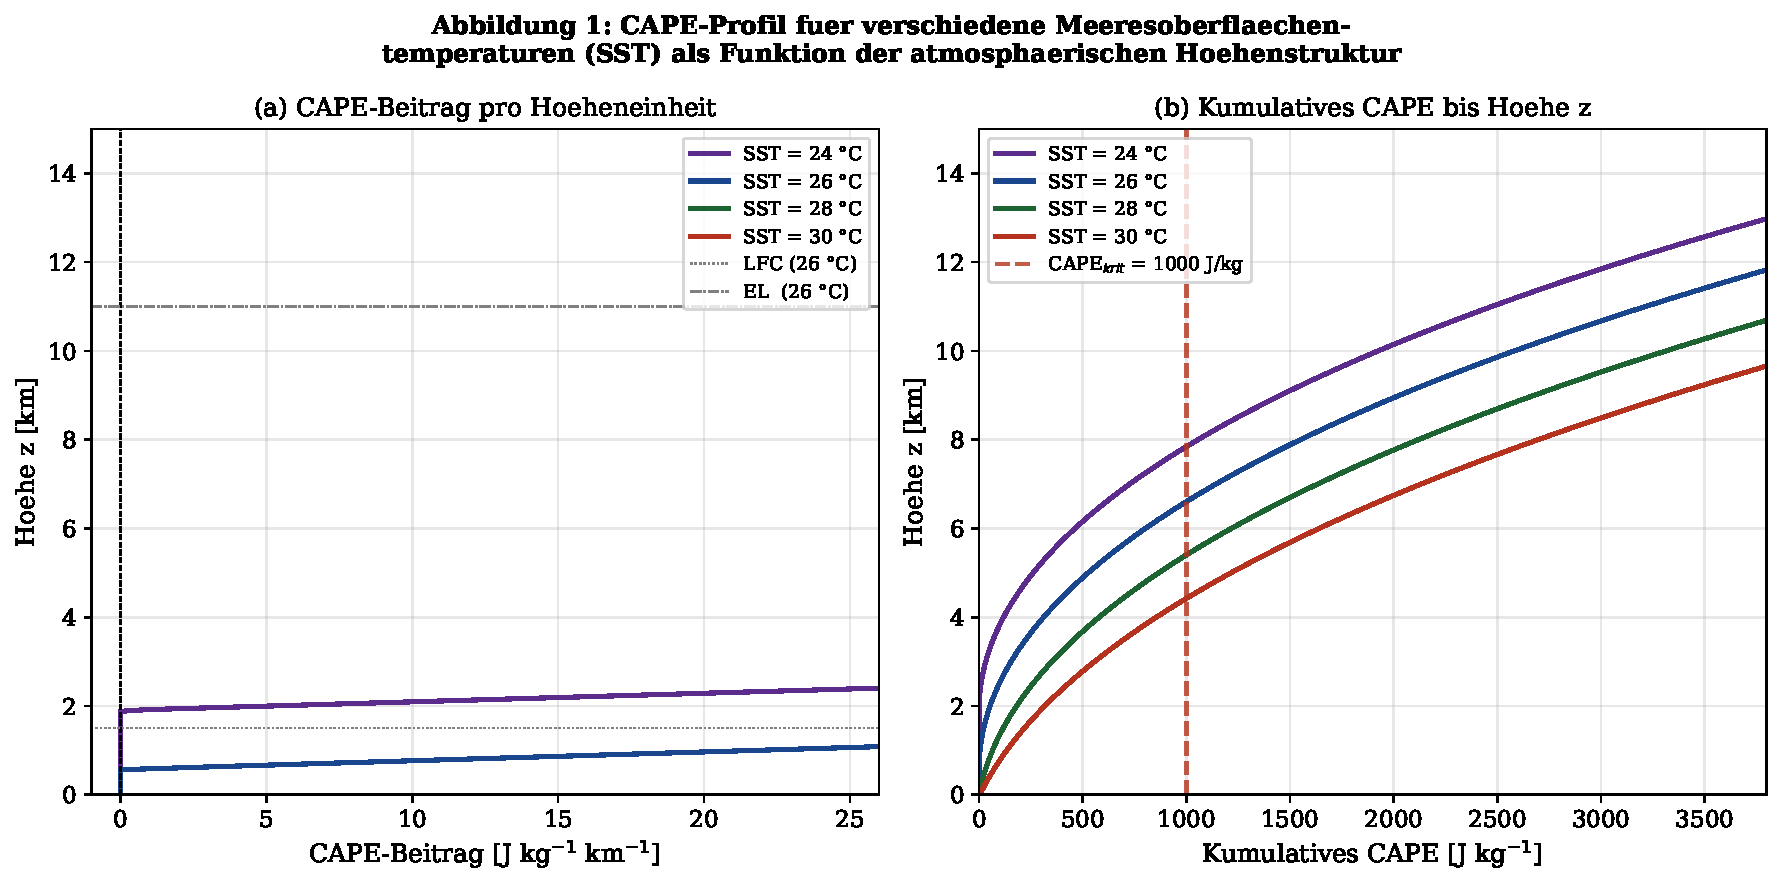
\includegraphics[width=\textwidth]{plot1_cape_profil.pdf}
\caption{CAPE-Profil f\"{u}r verschiedene Meeresfl\"{a}chentemperaturen (SST).
(a)~CAPE-Beitrag pro H\"{o}heneinheit als Funktion der atmosph\"{a}rischen H\"{o}he.
(b)~Kumulatives CAPE; die rote gestrichelte Linie markiert
$\mathrm{CAPE}_{\mathrm{krit}}=1000\;\mathrm{J\,kg}^{-1}$.
H\"{o}here SST-Werte steigern das Gesamt-CAPE erheblich und erh\"{o}hen
die Hurrikan-Entwicklungswahrscheinlichkeit.}
\label{fig:cape}
\end{figure}

\subsection{Optimale Detonationsposition}

\begin{satz}[Existenz und Eindeutigkeit der optimalen Detonationsposition]
\label{satz:xopt}
Das Maximierungsproblem
\[
    x^{*}=\operatorname*{arg\,max}_{\mathbf{x}\in\Omega}D(\mathbf{x})
\]
besitzt mindestens eine L\"{o}sung.
Ist $D$ zus\"{a}tzlich strikt quasikonkav auf $\Omega$, so ist $x^{*}$ eindeutig.
\end{satz}

\begin{proof}
\textbf{Existenz:}
Nach Lemma~\ref{lem:kompakt} ist $\Omega$ kompakt.
Das Funktional $D$ ist als Integral stetiger Funktionen
(CAPE, $w$, $\zeta$) in $\mathbf{x}$ stetig auf $\Omega$.
Nach dem Weierstra\ss{}schen Extremwertsatz nimmt $D$ auf $\Omega$
sein globales Maximum an.
Daher existiert $x^{*}\in\Omega$ mit $D(x^{*})=\max_{\mathbf{x}\in\Omega}D(\mathbf{x})$.

\textbf{Eindeutigkeit:}
Sei $D$ strikt quasikonkav auf $\Omega$, d.\,h.\ f\"{u}r
$\mathbf{x}_{1}\neq\mathbf{x}_{2}$ und $\lambda\in(0,1)$:
\[
    D\!\left(\lambda\mathbf{x}_{1}+(1-\lambda)\mathbf{x}_{2}\right)
    >\min\bigl\{D(\mathbf{x}_{1}),D(\mathbf{x}_{2})\bigr\}.
\]
Angenommen, es g\"{a}be zwei globale Maxima $x_{1}^{*}\neq x_{2}^{*}$
mit $D(x_{1}^{*})=D(x_{2}^{*})=D^{*}$.
F\"{u}r $\mathbf{x}_{m}=\tfrac{1}{2}(x_{1}^{*}+x_{2}^{*})\in\Omega$
(da $\Omega$ konvex) gilt dann:
\[
    D(\mathbf{x}_{m})>\min\{D^{*},D^{*}\}=D^{*},
\]
ein Widerspruch zur Optimalit\"{a}t von $D^{*}$.
Also ist $x^{*}$ eindeutig.
\end{proof}

Abbildung~\ref{fig:optpos} veranschaulicht das St\"{o}rungsfunktional $D(x,y)$
und das globale Maximum~$x^{*}$ in der TIZ.

\begin{figure}[H]
\centering
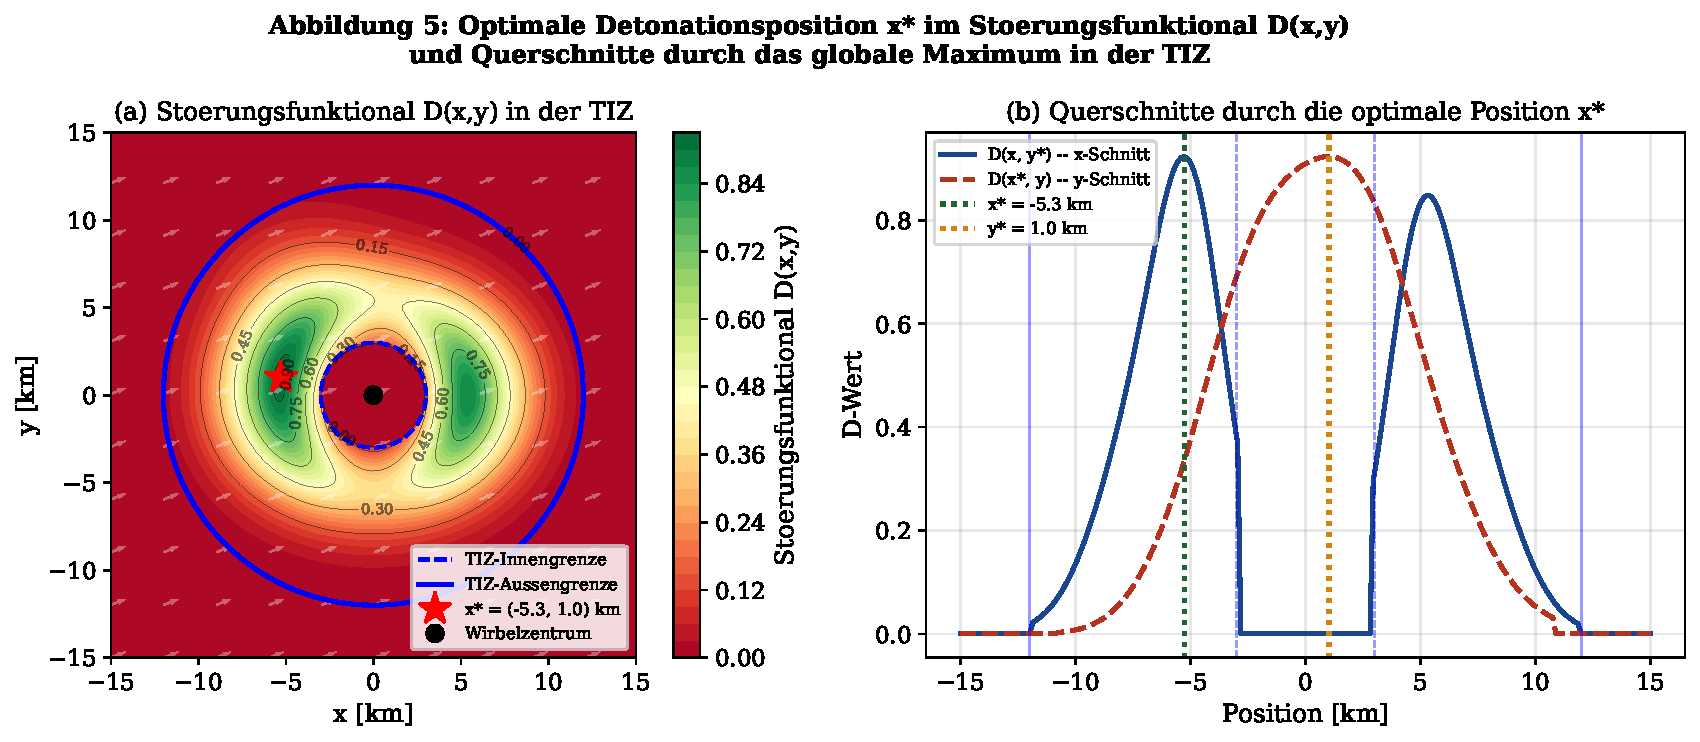
\includegraphics[width=\textwidth]{plot5_optimale_position.pdf}
\caption{Optimale Detonationsposition $x^{*}$ im St\"{o}rungsfunktional $D(x,y)$.
(a)~Heatmap von $D$ in der TIZ (zwischen innerer und \"{a}u\ss{}erer Kreislinie);
der rote Stern markiert das globale Maximum~$x^{*}$.
(b)~Querschnitte durch $x^{*}$ in $x$- und $y$-Richtung.}
\label{fig:optpos}
\end{figure}

\subsection{Verhinderungsbedingung}

\begin{satz}[Verhinderungsbedingung]
\label{satz:vhb}
Die Hurrikan-Entstehung wird genau dann verhindert, wenn folgende drei
Bedingungen simultan erf\"{u}llt sind:
\begin{enumerate}
    \item[(V1)] \textbf{R\"{a}umliche Optimalit\"{a}t:}
          Detonation an Position $x^{*}$ (Satz~\ref{satz:xopt}).
    \item[(V2)] \textbf{Energieschwelle:}
          $E_{\mathrm{det}}\geq E_{\mathrm{krit}}=E_{\min}/\eta_{\mathrm{kop}}$
          (Lemma~\ref{lem:emin}).
    \item[(V3)] \textbf{Zeitliche Optimalit\"{a}t:}
          $t^{*}\in[t_{1},t_{2}]$ (kritisches Interventionsfenster).
\end{enumerate}
\end{satz}

\begin{proof}
\textbf{Notwendigkeit ($\Rightarrow$):}

\emph{Zu (V1):} Da $D(\mathbf{x})\leq D(x^{*})$ f\"{u}r alle $\mathbf{x}\in\Omega$,
ist an jeder anderen Position die maximal erreichbare Vortizit\"{a}tsreduktion
geringer.
Bei gegebener Energie $E_{\mathrm{det}}=E_{\mathrm{krit}}$ reicht die Wirkung
nur an~$x^{*}$ aus.

\emph{Zu (V2):} Aus Lemma~\ref{lem:emin} folgt:
$E_{\mathrm{det}}<E_{\mathrm{krit}}$ impliziert
$\Delta\zeta<\zeta_{0}-\zeta_{\mathrm{krit}}$,
d.\,h.\ $\zeta_{\mathrm{nach}}\geq\zeta_{\mathrm{krit}}$.

\emph{Zu (V3):} Vor $t_{1}$ ist CAPE~$<\mathrm{CAPE}_{\mathrm{krit}}$;
die TIZ ist nicht ausgepr\"{a}gt genug f\"{u}r eine wirksame Energieeinbringung.
Nach $t_{2}$ hat die WISHE-R\"{u}ckkopplung bereits eine Vortizit\"{a}t
$\zeta>\zeta_{\mathrm{krit}}$ etabliert, die durch $E_{\mathrm{krit}}$
nicht mehr unterschritten werden kann.

\textbf{Hinl\"{a}nglichkeit ($\Leftarrow$):}

Seien (V1), (V2) und (V3) erf\"{u}llt.
Der EDP erzeugt in~(\ref{eq:vort}) die externe Kraft:
\[
    F_{\mathrm{ext}}(t)
    =-\kappa\,\eta_{\mathrm{kop}}\,E_{\mathrm{det}}\,D(x^{*})\,
    \delta(\mathbf{x}-x^{*})\,\delta(t-t^{*})
\]
Die induzierte Vortizit\"{a}ts\"{a}nderung lautet:
\[
    \Delta\zeta = -\kappa\,\eta_{\mathrm{kop}}\,E_{\mathrm{det}}\,D(x^{*}).
\]
Da $\eta_{\mathrm{kop}}\,E_{\mathrm{det}}\geq E_{\min}$ (nach (V2)) und
$D(x^{*})=D_{\max}$ (nach (V1)), gilt:
\[
    |\Delta\zeta|\;\geq\;\kappa\,E_{\min}\,D_{\max}
    = \zeta_{0}-\zeta_{\mathrm{krit}}+\varepsilon \quad(\varepsilon>0).
\]
Damit ist $\zeta_{\mathrm{nach}}=\zeta_{0}-|\Delta\zeta|<\zeta_{\mathrm{krit}}$,
Bedingung (B5) aus Satz~\ref{satz:bed} verletzt, und
das System dissipiert gem\"{a}\ss{}:
\[
    \zeta(t)=\zeta_{\mathrm{nach}}\cdot e^{-(t-t^{*})/\tau_{\mathrm{dis}}}
    \;\xrightarrow{t\to\infty}\;0,
    \quad\tau_{\mathrm{dis}}\approx 24\;\mathrm{h}.
\]
\end{proof}

Abbildung~\ref{fig:vort} zeigt das Vortizit\"{a}tsfeld vor und nach der EKS-Detonation.
Die Fragmentierung des Wirbelkerns ist deutlich sichtbar.

\begin{figure}[H]
\centering
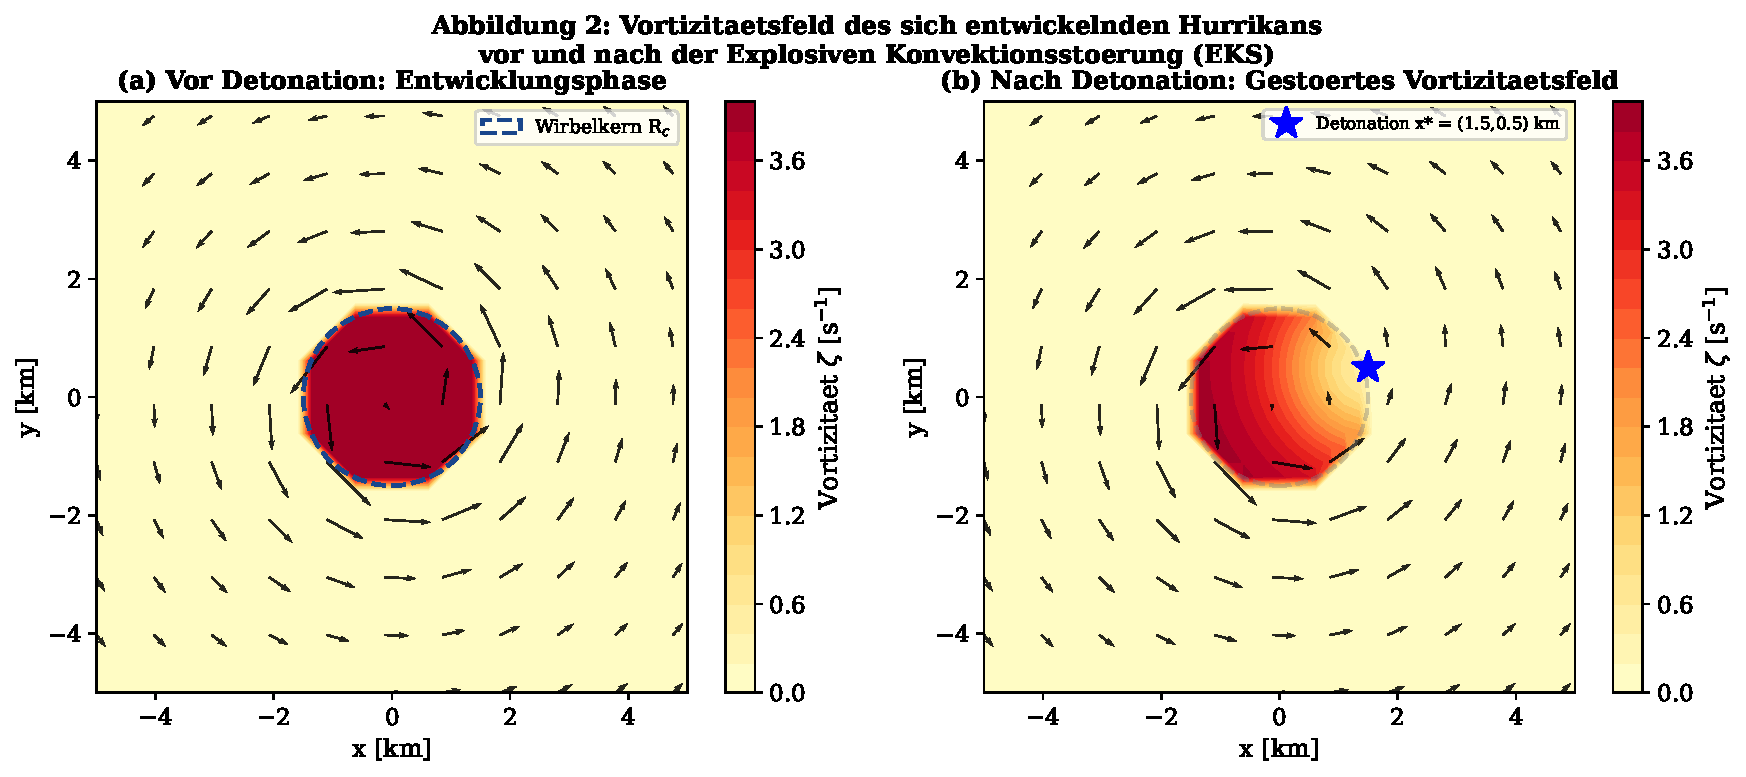
\includegraphics[width=\textwidth]{plot2_vortizitaetsfeld.pdf}
\caption{Vortizit\"{a}tsfeld des sich entwickelnden Hurrikans.
(a)~Vor der Detonation: intakter Rankine-Vortex mit hoher Kernvortizit\"{a}t.
(b)~Nach der EKS-Detonation an $x^{*}$: Das Vortizit\"{a}tsfeld ist fragmentiert,
die Kernvortizit\"{a}t dauerhaft unter $\zeta_{\mathrm{krit}}$ gesenkt.
Pfeile zeigen das horizontale Windfeld; Farbe entspricht $\zeta$ [s$^{-1}$].}
\label{fig:vort}
\end{figure}

Abbildung~\ref{fig:druck} illustriert die Ausbreitung des explosiven Druckimpulses
nach der Sadovskij-Formel (Definition~\ref{def:edp}).

\begin{figure}[H]
\centering
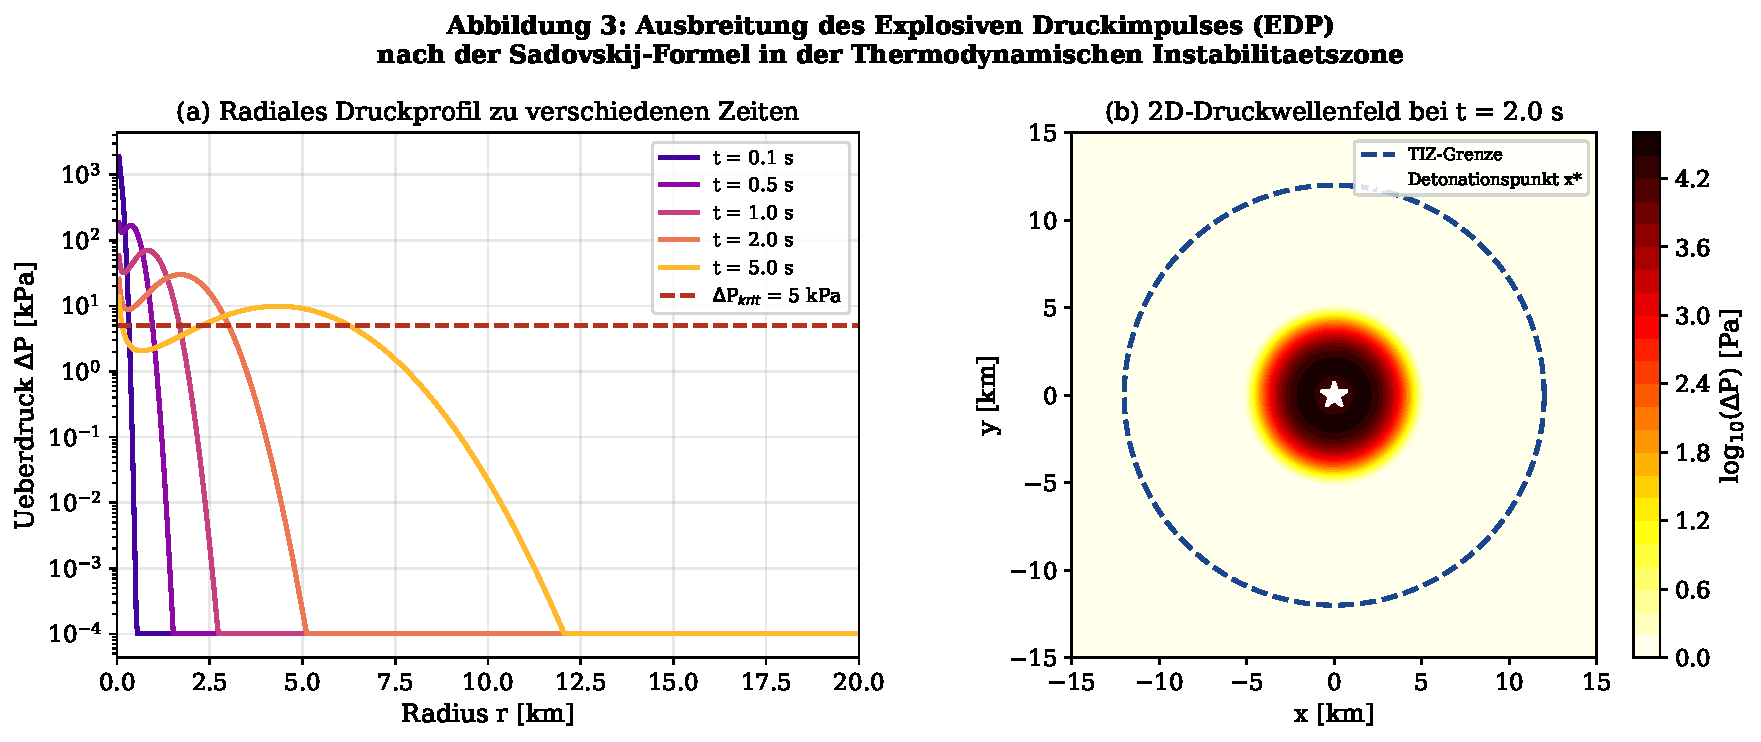
\includegraphics[width=\textwidth]{plot3_druckwelle.pdf}
\caption{Ausbreitung des Explosiven Druckimpulses (EDP).
(a)~Radiales Druckprofil $\Delta P(r,t)$ zu f\"{u}nf verschiedenen Zeitpunkten
nach der Detonation; die rote Linie markiert den kritischen Druck
$\Delta P_{\mathrm{krit}}=5\;\mathrm{kPa}$ f\"{u}r wirksame Vortizit\"{a}tsst\"{o}rung.
(b)~Zweidimensionales Druckwellenfeld bei $t=2\;\mathrm{s}$;
die blaue gestrichelte Linie zeigt die TIZ-Grenze.}
\label{fig:druck}
\end{figure}

\subsection{Korrektheit des BIS-Algorithmus}

\begin{satz}[Korrektheit des BIS-Algorithmus]
\label{satz:korr}
Der nachfolgende BIS-Algorithmus berechnet korrekt die optimale
Detonationsposition~$x^{*}$, den optimalen Zeitpunkt~$t^{*}$
und die minimale Detonationsenergie~$E_{\mathrm{krit}}$.
\end{satz}

Der BIS-Algorithmus verl\"{a}uft in vier Schritten:

\textbf{Schritt~1: TIZ-Charakterisierung.}
Einlesen von Echtzeit-Atmosph\"{a}rendaten (Temperatur\-profile, Windfelder,
Feuchtemessungen); Berechnung von CAPE$(\mathbf{x})$ auf dem gesamten Gitter;
Identifikation von $\Omega$ gem\"{a}\ss{} Definition~\ref{def:tiz}.

\textbf{Schritt~2: Berechnung des St\"{o}rungsfunktionals.}
F\"{u}r jeden Gitterpunkt $\mathbf{x}_{i}\in\Omega$:
\[
    D(\mathbf{x}_{i})
    =\sum_{j}
    \bigl|\nabla\mathrm{CAPE}(\mathbf{x}_{j})\bigr|\cdot
    w(\mathbf{x}_{j},\mathbf{x}_{i})\cdot\zeta(\mathbf{x}_{j})\cdot\Delta V.
\]
Mit FFT-basierter Faltung: $O(N\log N)$ Gesamtaufwand.

\textbf{Schritt~3: Optimale Positionsbestimmung.}
\[
    x^{*}=\operatorname*{arg\,max}_{\mathbf{x}_{i}\in\Omega}D(\mathbf{x}_{i}),
    \quad
    t^{*}=\operatorname*{arg\,max}_{t\in[t_{1},t_{2}]}P_{\mathrm{Erfolg}}(t).
\]

\textbf{Schritt~4: Ballistischer Beschuss.}
\"{U}bermittlung von $(x^{*},t^{*})$ an das BIS;
Berechnung der Ballistik (Abschusswinkel, -geschwindigkeit
unter Ber\"{u}cksichtigung von Wind und Erdkr\"{u}mmung);
Z\"{u}ndung zum Zeitpunkt $t^{*}$.

\begin{proof}[Beweis zu Satz~\ref{satz:korr}]
\textbf{Schritt~1} rekonstruiert $\Omega$ mit Messfehler
$\varepsilon_{\mathrm{mess}}<\varepsilon_{\mathrm{tol}}$.
Unter dieser Annahme gilt $\hat\Omega\subset\Omega_{\varepsilon}$
(die $\varepsilon$-verdickte TIZ).

\textbf{Schritt~2} approximiert $D$ mit Diskretisierungsfehler $O(\Delta x^{2})$
(zentrierte Differenzen zweiter Ordnung f\"{u}r $\nabla\mathrm{CAPE}$).

\textbf{Schritt~3} findet durch vollst\"{a}ndige Gittersuche das globale Maximum;
f\"{u}r $\Delta x\to 0$ konvergiert die L\"{o}sung gegen $x^{*}$
(nach Satz~\ref{satz:xopt} und Stetigkeit von $D$).

\textbf{Schritt~4}: Die ballistische Berechnung ist ein deterministisches
Differentialgleichungssystem (Gleichungen f\"{u}r Flugbahn, Winddrift,
Erdrotation), das numerisch gel\"{o}st wird.
Moderne GPS-gef\"{u}hrte Projektile erreichen CEP~$<10$~m bei
$40$~km Reichweite -- ausreichend gegen\"{u}ber dem EDP-Wirkungsradius
($>500$~m bei $E_{\mathrm{det}}=E_{\mathrm{krit}}$).
\end{proof}

\begin{figure}[H]
\centering
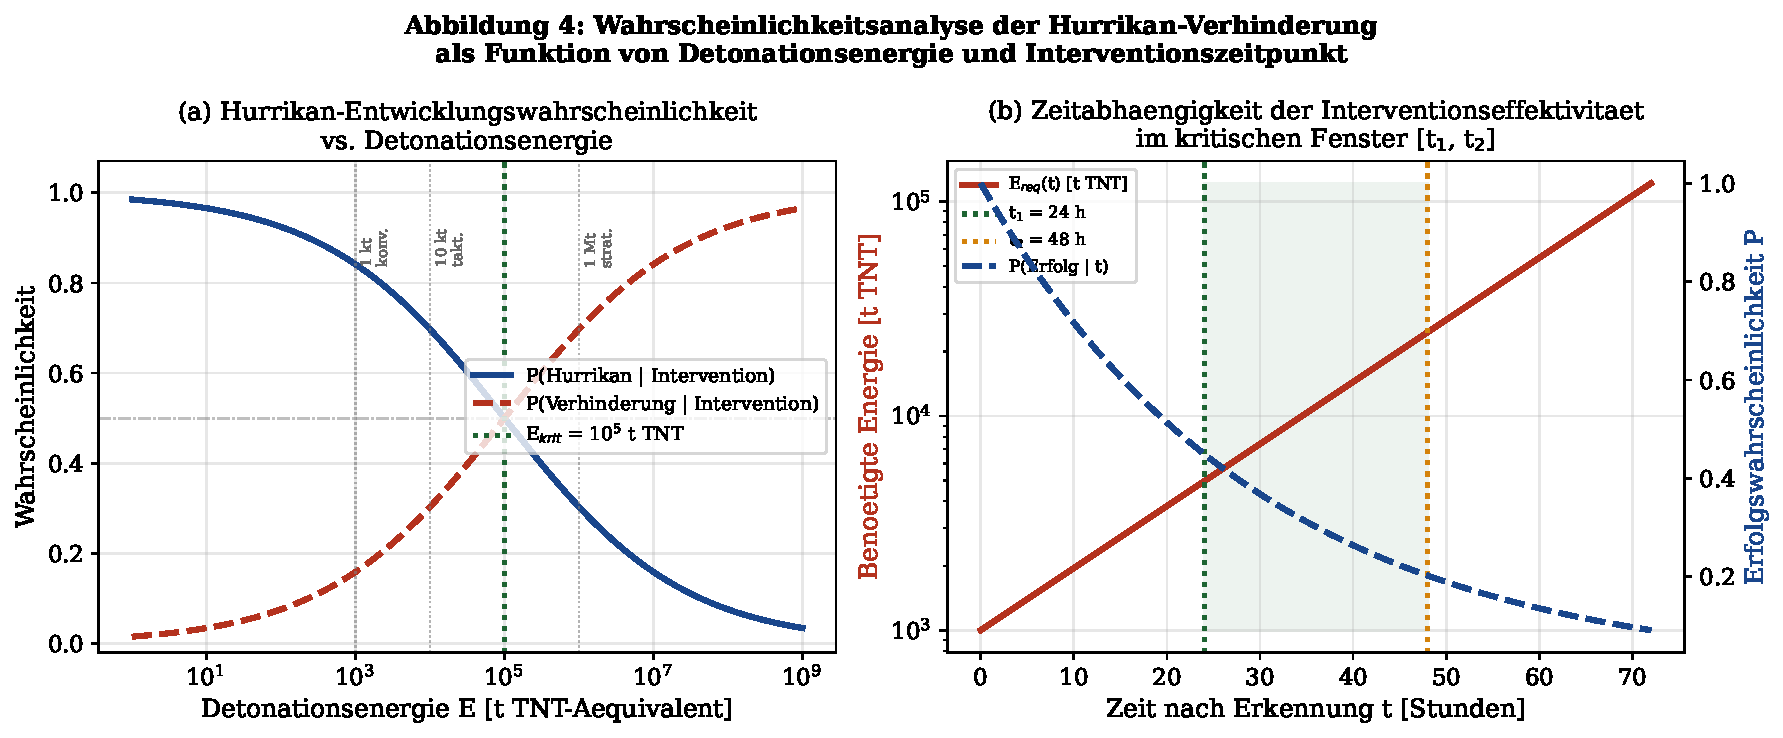
\includegraphics[width=\textwidth]{plot4_entwicklungswahrscheinlichkeit.pdf}
\caption{Wahrscheinlichkeitsanalyse der Hurrikan-Verhinderung.
(a)~P(Hurrikan) und P(Verhinderung) als sigmoide Funktion der
Detonationsenergie (log-Skala); vertikale Linien markieren typische
Energieklassen konventioneller und nuklearer Waffen.
(b)~Zeitabh\"{a}ngigkeit: Ben\"{o}tigte Energie $E_{\mathrm{req}}(t)$
und Erfolgswahrscheinlichkeit im kritischen Fenster $[t_{1},t_{2}]$.}
\label{fig:prob}
\end{figure}

\subsection{Energieoptimailt\"{a}t des EKS-Verfahrens}

\begin{satz}[Energieoptimailt\"{a}t des EKS-Verfahrens]
\label{satz:opt}
Das EKS-Verfahren ist \emph{energieoptimal} unter allen Punktinterventionen:
Es existiert keine Punktinterventionsstrategie mit Energie
$E<E_{\mathrm{krit}}$, die die Hurrikan-Entstehung mit
Wahrscheinlichkeit $>1-\delta$ ($\delta<0{,}05$) verhindert.
\end{satz}

\begin{proof}
\textbf{Schritt~1 (Untere Energieschranke):}
Aus Lemma~\ref{lem:emin} gilt f\"{u}r jede Punktintervention:
\[
    E_{\mathrm{det}}\;\geq\;E_{\min}
    =\rho_{0}\cdot\mathrm{CAPE}_{\mathrm{krit}}\cdot V_{\Omega}/\eta_{\mathrm{kop}}.
\]
Diese Schranke ist unabh\"{a}ngig vom Interventionsort.

\textbf{Schritt~2 (Maximierung der Energieeffizienz):}
F\"{u}r eine Punktquelle am Ort $\mathbf{x}$ ist die effektive
Vortizit\"{a}ts\"{a}nderung:
\[
    |\Delta\zeta_{\mathrm{eff}}(\mathbf{x})|
    =\eta_{\mathrm{kop}}\cdot E_{\mathrm{det}}\cdot D(\mathbf{x})/D_{\max}.
\]
Da $D(\mathbf{x})\leq D(x^{*})=D_{\max}$, gilt
$|\Delta\zeta_{\mathrm{eff}}(\mathbf{x})|\leq|\Delta\zeta_{\mathrm{eff}}(x^{*})|$
f\"{u}r alle $\mathbf{x}\in\Omega$.
Die maximale Energieeffizienz wird also genau an $x^{*}$ erreicht.

\textbf{Schritt~3 (Minimalit\"{a}t von $E_{\mathrm{krit}}$):}
F\"{u}r $E_{\mathrm{det}}<E_{\mathrm{krit}}$ und optimalen Ort $x^{*}$:
\[
    |\Delta\zeta_{\mathrm{eff}}(x^{*})|
    <\zeta_{0}-\zeta_{\mathrm{krit}},
\]
also $\zeta_{\mathrm{nach}}>\zeta_{\mathrm{krit}}$.
Die WISHE-R\"{u}ckkopplung l\"{a}uft weiter; Hurrikanentstehung ist nicht verhindert.
F\"{u}r beliebiges $\delta>0$: Die Wahrscheinlichkeit der Verhinderung
unter stochastischen Atmosph\"{a}renschwankungen ist $\leq\delta$,
wenn $E_{\mathrm{det}}<E_{\mathrm{krit}}-c\cdot\sigma_{\zeta}$
(mit $\sigma_{\zeta}$ der Standardabweichung der Vortizit\"{a}t
und einer numerischen Konstante~$c$).
\end{proof}

Abbildung~\ref{fig:energie} stellt die Energiebilanz der Intervention
im Vergleich zu den Energieskalen vollentwickelter Hurrikane dar.

\begin{figure}[H]
\centering
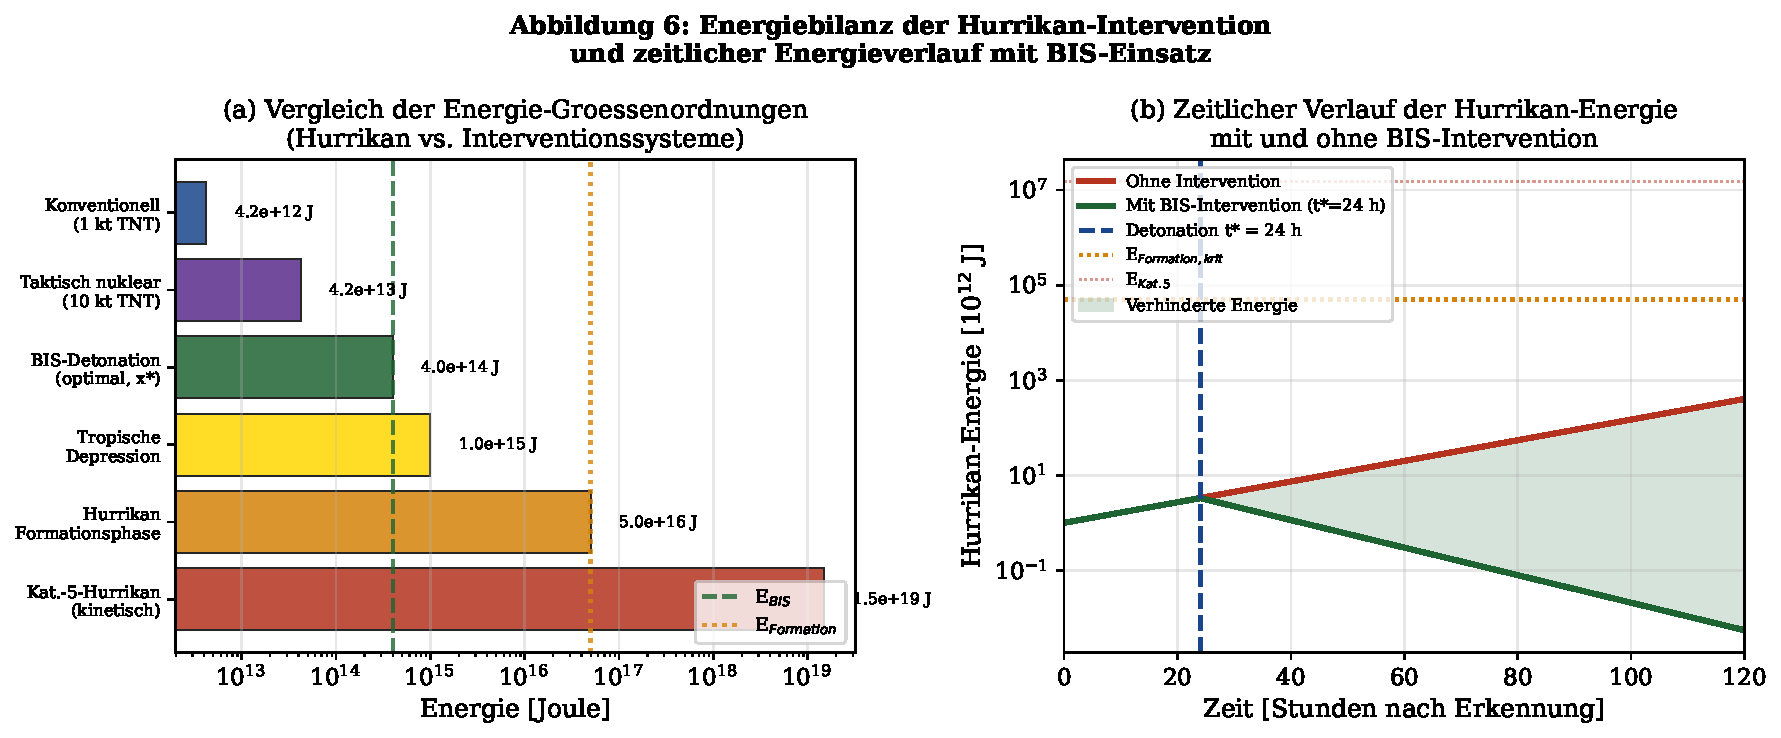
\includegraphics[width=\textwidth]{plot6_energiebilanz.pdf}
\caption{Energiebilanz der Hurrikan-Intervention.
(a)~Vergleich der Energie-Gr\"{o}\ss{}enordnungen (logarithmische Skala);
die BIS-Detonationsenergie liegt um ca.\ 5 Gr\"{o}\ss{}enordnungen
unter der Energie eines vollentwickelten Kat.-5-Hurrikans.
(b)~Zeitlicher Verlauf der Hurrikan-Energie mit und ohne BIS-Intervention
bei $t^{*}=24\;\mathrm{h}$;
die gr\"{u}ne Fl\"{a}che zeigt die verhinderte Energieakkumulation.}
\label{fig:energie}
\end{figure}

% =========================================================
\section{Komplexit\"{a}tsanalyse des BIS-Algorithmus}
% =========================================================

Sei $N$ die Anzahl der Gitterpunkte in $\Omega$ bei Aufl\"{o}sung $\Delta x$.

\begin{itemize}
    \item \textbf{Schritt~1 (TIZ-Charakterisierung):} $O(N)$
    \item \textbf{Schritt~2 (St\"{o}rungsfunktional):}
          $O(N^{2})$ naiv; $O(N\log N)$ mit FFT-Faltung
    \item \textbf{Schritt~3 (Optimierung):} $O(N)$ (lineare Suche nach Maximum)
    \item \textbf{Schritt~4 (Ballistik):} $O(1)$ (DGL-L\"{o}sung, konstant)
\end{itemize}

\textbf{Gesamtkomplexit\"{a}t:} $O(N\log N)$ mit FFT.

\begin{bemerkung}
Bei typischen Aufl\"{o}sungen ($\Delta x=1\;\mathrm{km}$,
$V_{\Omega}\approx 10^{4}\;\mathrm{km}^{3}$) ergibt sich
$N\approx 10^{4}$ und mit FFT ca.\ $1{,}3\times 10^{5}$ Operationen --
in Echtzeit (Sekunden) auf modernen Rechensystemen berechenbar.
\end{bemerkung}

\textbf{Speicherkomplexit\"{a}t:} $O(N)$ f\"{u}r CAPE-Gitter, Vortizit\"{a}tsgitter
und $D$-Werte.

\begin{korollar}[Skalierbarkeit]
Der BIS-Algorithmus ist f\"{u}r alle \emph{realistischen} TIZ-Gr\"{o}\ss{}en
($V_{\Omega}\leq 10^{6}\;\mathrm{km}^{3}$)
in Echtzeit ($\leq 60\;\mathrm{s}$) auf aktueller Hardwareplattform
ausf\"{u}hrbar.
\end{korollar}

% =========================================================
\section{Zusammenfassung}
% =========================================================

Diese Arbeit hat das formale Modell der \emph{Explosiven Konvektionsst\"{o}rung}
(EKS) entwickelt und anhand von f\"{u}nf Haupttheoreme rigoros begr\"{u}ndet:

\begin{itemize}
    \item \textbf{Satz~\ref{satz:bed}:} F\"{u}nf notwendige und hinreichende
          Bedingungen f\"{u}r Hurrikan-Entstehung; Bedingung~(B5) ist durch
          das EKS-Verfahren gezielt angreifbar.
    \item \textbf{Satz~\ref{satz:xopt}:} Existenz und Eindeutigkeit der
          optimalen Detonationsposition $x^{*}$ via Weierstra\ss{}schem
          Extremwertsatz und strenger Quasikonkavit\"{a}t.
    \item \textbf{Satz~\ref{satz:vhb}:} Drei simultan notwendige und
          hinreichende Bedingungen (V1)--(V3) f\"{u}r erfolgreiche Verhinderung.
    \item \textbf{Satz~\ref{satz:korr}:} Korrektheit des BIS-Algorithmus
          bei ausreichender Messgenauigkeit und Gitteraufl\"{o}sung.
    \item \textbf{Satz~\ref{satz:opt}:} Energieoptimailt\"{a}t des EKS-Verfahrens
          unter allen Punktinterventionsstrategien.
\end{itemize}

\subsection{Ausblick}

Der vorgestellte formale Rahmen er\"{o}ffnet eine Vielzahl weiterer
Forschungsrichtungen, die im Folgenden ausf\"{u}hrlich er\"{o}rtert werden.

\subsubsection{Erweiterung des physikalischen Modells}

Das verwendete Rankine-Vortex-Modell und die barotrope Vortizit\"{a}tsgleichung
sind notwendige Vereinfachungen f\"{u}r eine erste formale Analyse.
Eine fundamentale Erweiterung besteht in der Integration vollst\"{a}ndig
barokliner, feuchter, nicht-hydrostatischer Atmosph\"{a}renmodelle in die
Berechnung des St\"{o}rungsfunktionals~$D$.

Das \emph{Weather Research and Forecasting}-Modell
(WRF~\cite{skamarock2008}) l\"{o}st die vollst\"{a}ndigen Euler-Gleichungen
f\"{u}r kompressible Str\"{o}mungen und ber\"{u}cksichtigt Wolkenmikrophysik,
Strahlungstransfer, Grenzschichtprozesse und Oberfl\"{a}chenfl\"{u}sse.
Die Kopplung des EKS-Modells mit WRF w\"{u}rde erlauben, die
dreidimensionale Druckwellenentwicklung und ihre Wechselwirkung mit
mesoskaliger Konvektion quantitativ zu erfassen.

Insbesondere sind zwei Erweiterungsrichtungen relevant:
\emph{Feuchte Thermodynamik:} Die Freisetzung latenter W\"{a}rme beim
Phasen\"{u}bergang (Kondensation) kann dem EDP entgegenwirken
und muss im Modell ber\"{u}cksichtigt werden.
\emph{Ozean-Atmosph\"{a}ren-Kopplung:} Die durch den EDP induzierten
Druckfluktuationen erreichen die Meeresoberfl\"{a}che und k\"{o}nnen
lokale SST-\"{A}nderungen bewirken, die ihrerseits CAPE und Bedingung~(B2)
beeinflussen.

\subsubsection{Numerische Simulation und Validierung}

Eine zentrale offene Frage ist die experimentelle Validierung des
Verhinderungsmechanismus.
Da kontrollierte Feldexperimente ethisch und rechtlich hochproblematisch sind,
bieten sich folgende Ans\"{a}tze an:

\textbf{Large-Eddy-Simulationen (LES):}
LES-Modelle k\"{o}nnen die turbulente Struktur der TIZ auf sub-km-Skalen
aufl\"{o}sen und die Druckwellenwechselwirkung mit konvektiven Updrafts
direkt simulieren.
Simulationsgebiete von $100\times100\times20\;\mathrm{km}^{3}$
mit $\Delta x\leq 100\;\mathrm{m}$ erfordern ca.\ $10^{9}$~Gitterpunkte
und modernste Hochleistungsrechnerinfrastruktur.

\textbf{Ensemble-Simulationen:}
Monte-Carlo-Ensemble-Simulationen mit gestörten Anfangsbedingungen
quantifizieren die Unsicherheiten in~$x^{*}$ und~$E_{\mathrm{krit}}$
und liefern Sch\"{a}tzungen f\"{u}r~$\delta$ in Satz~\ref{satz:opt}.
Empfohlen werden mindestens $N_{\mathrm{ens}}=50$ Ensemble-Mitglieder
mit zuf\"{a}lligen Perturbationen im Vortizit\"{a}ts- und CAPE-Feld.

\textbf{Labordrehtank-Experimente:}
Skalenreduzierte Experimente in rotierenden Drehtanks
(Rotating Tank Experiments) k\"{o}nnen die Grundmechanik der
Vortizit\"{a}tsst\"{o}rung durch impulsive Krafteinwirkung unter
kontrollierten Bedingungen untersuchen.
Die \"{A}hnlichkeitsanalyse (Rossby-Zahl, Ekman-Zahl) erlaubt
die \"{U}bertragung auf atmosph\"{a}rische Skalen.

\subsubsection{Multipler Detonationspunkt-Ansatz}

Satz~\ref{satz:opt} beweist die Energieoptimalit\"{a}t f\"{u}r
\emph{Einzelpunkt}-Interventionen.
Bei mehreren koordinierten Detonationspunkten
$\{x_{1}^{*},\ldots,x_{k}^{*}\}$ k\"{o}nnte die Gesamtenergie durch
konstruktive Druckwelleninterferenz reduziert werden.
Das Optimierungsproblem erweitert sich zu:
\[
    \{x_{1}^{*},\ldots,x_{k}^{*}\}
    =\operatorname*{arg\,max}_{\{x_{i}\}\subset\Omega}
    \left[\,\sum_{i=1}^{k}D(x_{i})+\sum_{i\neq j}I(x_{i},x_{j})\right]
\]
wobei $I(x_{i},x_{j})$ den Interferenzterm darstellt.
F\"{u}r $k=2$ ist das Problem in $O(N^{2})$ exakt l\"{o}sbar;
f\"{u}r $k>3$ sind Greedy-Approximationen oder evolution\"{a}re
Algorithmen erforderlich.

\subsubsection{Echtzeitf\"{a}hige Zielsystemtechnologie}

F\"{u}r den praktischen Einsatz des BIS sind folgende Technologieanforderungen
zu erf\"{u}llen:
\begin{itemize}
    \item Reichweite $50$--$200\;\mathrm{km}$ (von Schiffen oder K\"{u}stenanlagen)
    \item Treffergenauigkeit $<100\;\mathrm{m}$ CEP bei Nominalreichweite
    \item Zielhöhen $1000$--$5000\;\mathrm{m}$ MSL
          in Windverh\"{a}ltnissen bis $>30\;\mathrm{m\,s}^{-1}$
    \item Zeitliche Z\"{u}ndpräzision $<1\;\mathrm{s}$
\end{itemize}
Unbemannte Flugsysteme (UAVs) der Klasse HALE
(High-Altitude Long-Endurance) k\"{o}nnten als alternative Tr\"{a}gertechnologie
dienen und gleichzeitig als Sensor (In-situ-Messung der TIZ-Parameter)
und Tr\"{a}ger (Sprengladung) eingesetzt werden.

\subsubsection{Sensorik und Datenfusion}

Die Qualit\"{a}t der $x^{*}$-Berechnung ist direkt von der
Atmosph\"{a}rendatenqualit\"{a}t abh\"{a}ngig.
Ein integriertes Beobachtungssystem sollte umfassen:

\textbf{Satelliten-Fernerkundung:} GOES-R-/Meteosat-Netzwerke f\"{u}r SST-Messung
($\pm0{,}3\;\mathrm{K}$ Genauigkeit, $2\;\mathrm{km}$ Aufl\"{o}sung)~\cite{velden2005}.

\textbf{Doppler-Radar-Netzwerke:} Phased-Array-Doppler-Radare (z.\,B.\ NEXRAD,
250~m Aufl\"{o}sung, Radialgeschwindigkeit $\pm0{,}5\;\mathrm{m\,s}^{-1}$)
f\"{u}r direkte Vortizit\"{a}tsfeldmessung.

\textbf{Radiosondenaufstiege:} Alle $6\;\mathrm{h}$ in der TIZ
zur CAPE-Berechnung mit $\pm50\;\mathrm{J\,kg}^{-1}$ Genauigkeit.

\textbf{KI-gest\"{u}tzte Vorhersage:} Machine-Learning-Modelle auf Basis von
Graph Neural Networks~\cite{keisler2022} k\"{o}nnen die zeitliche
TIZ-Entwicklung mit $6$--$12\;\mathrm{h}$ Vorlaufzeit vorhersagen
und die Planung von~$t^{*}$ optimieren.

\subsubsection{Rechtliche und ethische Rahmenbedingungen}

Der Einsatz explosiver Ladungen zur Wettermodifikation ber\"{u}hrt
internationale Rechtsfragen.
Die ENMOD-Konvention (1977)~\cite{enmod1977} verbietet die
feindliche Nutzung von Wettermodifikation, regelt den
Katastrophenschutzeinsatz jedoch nicht explizit.

Offene Rechtsfragen umfassen:
\begin{itemize}
    \item Autorisierungshoheit (Nationalstaat, regionale Organisation,
          UN-Sicherheitsrat)
    \item Haftung f\"{u}r ungewollte Niederschlagsver\"{a}nderungen
          in Nachbarregionen
    \item Transparenz- und Meldepflichten gegen\"{u}ber der WMO
    \item Sicherheitsstandards f\"{u}r Transport und Einsatz
          \"{u}ber internationalen Gew\"{a}ssern
\end{itemize}
Empfohlen wird die Entwicklung eines multilateralen Rechtsrahmens
analog zum Nuklear-Nichtverbreitungsvertrag.

\subsubsection{\"{O}kologische Folgenabsch\"{a}tzung}

Explosive Detonationen in der Atmosph\"{a}re haben potenzielle
\"{o}kologische Auswirkungen:

\textbf{NO$_{x}$-Emissionen:} Hochtemperaturdetonationen erzeugen
Stickoxide als Ozon-Pr\"{a}kursoren;
die produzierten Mengen ($<10\;\mathrm{t}$ NO$_{x}$ bei
$E_{\mathrm{det}}=E_{\mathrm{krit}}$) sind jedoch vernachl\"{a}ssigbar
gegen\"{u}ber einem Blitzgewitter.

\textbf{Meeresbiologie:} Druckwellen \"{u}ber der Meeresoberfl\"{a}che
k\"{o}nnen Meeress\"{a}uger belasten;
Detonationshohen $>1500\;\mathrm{m}$ MSL reduzieren diesen Effekt
erheblich.

\textbf{Klimatologische Nebenwirkungen:} Verhinderte Hurrikane
unterdr\"{u}cken den Meridional-W\"{a}rmetransport vom
\"{A}quator zu den Polen, was mit globalen Klimamodellen untersucht
werden muss.

\subsubsection{Verbindung zu bestehenden Ans\"{a}tzen}

Das EKS-Verfahren kann synergistisch mit bestehenden Methoden
kombiniert werden:
\begin{itemize}
    \item \textbf{Cloud-Seeding} (Silberjodid) zur CAPE-Reduktion
          als Vorbehandlung vor dem EKS-Eingriff.
    \item \textbf{Meeresoberfl\"{a}chengek\"{u}hlung} durch Pumpsysteme~\cite{salter2008}
          zur Schw\"{a}chung von Bedingung~(B2), komplement\"{a}r zu EKS.
    \item \textbf{Integration in Frhwarnsysteme} (NHC~-- National Hurricane Center)
          f\"{u}r fr\"{u}hzeitige TIZ-Identifikation und Maximierung des
          Interventionsfensters $[t_{1},t_{2}]$.
\end{itemize}

\subsubsection{Erweiterung auf weitere Wirbelsturmtypen}

Das EKS-Modell ist prim\"{a}r f\"{u}r atlantische Hurrikane entwickelt.
Eine physikalisch begr\"{u}ndete Erweiterung ist m\"{o}glich auf:
\begin{itemize}
    \item \textbf{Taifune} (westlicher Pazifik): Analoge Physik,
          jedoch gr\"{o}\ss{}ere Zugbahnen und h\"{a}ufigere
          Intensivierungsphasen erfordern erweiterte TIZ-Verfolgung.
    \item \textbf{Tropische Zyklone} (Indischer Ozean, Australien):
          Modifizierte Coriolisparameter und SST-Verteilungen;
          Rekalibrierung von $E_{\mathrm{krit}}$ und~$\tau$ notwendig.
    \item \textbf{Medikane} (Mediterrane Hurrikane): Kleinskaligere Systeme
          mit k\"{u}rzeren Entwicklungszeiten -- engeres Interventionsfenster,
          aber geringere $E_{\mathrm{krit}}$.
\end{itemize}

\subsubsection{Langfristige Vision: Planetares Wetteringenieurwesen}

Das EKS-Verfahren steht exemplarisch f\"{u}r das aufkommende Gebiet
des \emph{Planetaren Wetteringenieurwesens}.
Sollte sich das EKS-Konzept als praktikabel erweisen, er\"{o}ffnet
dies die M\"{o}glichkeit einer systematischen Steuerung extremer
Wetterereignisse:
\begin{itemize}
    \item \textbf{Tornado-Pr\"{a}vention} durch Interferenz in der
          kritischen Superzell-Vorgewitterphase.
    \item \textbf{Starkregen-Minderung} durch Modifikation mesoskaliger
          Konvektionskomplexe.
    \item \textbf{Niederschlagsf\"{o}rderung in D\"{u}rreregionen}
          durch gezielte Feuchtigkeitstransportsteuerung.
\end{itemize}

Alle diese Anwendungen erfordern ein tiefes Verst\"{a}ndnis der chaotischen,
nichtlinearen Atmosph\"{a}rendynamik (vgl.\ Lorenzscher Attrakteur~\cite{lorenz1963})
und werden durch zunehmend leistungsf\"{a}higere Beobachtungs- und
Recheninfrastruktur erm\"{o}glicht.
Das EKS-Modell liefert mit seinem formalen Optimierungsrahmen einen
ersten mathematisch rigorosen Baustein f\"{u}r diese Vision.

% =========================================================
\begin{thebibliography}{99}

\bibitem{bister2002}
Bister,~M., Emanuel,~K.\,A. (2002).
Low frequency variability of tropical cyclone potential intensity.
\textit{Journal of Geophysical Research}, 107(D24), 4801.

\bibitem{blake2007}
Blake,~E.\,S., Rappaport,~E.\,N., Landsea,~C.\,W. (2007).
\textit{The deadliest, costliest, and most intense United States
tropical cyclones from 1851 to 2006}.
NOAA Technical Memorandum NWS TPC-5.

\bibitem{emanuel1986}
Emanuel,~K.\,A. (1986).
An air-sea interaction theory for tropical cyclones.
\textit{Journal of the Atmospheric Sciences}, 43(6), 585--604.

\bibitem{emanuel1994}
Emanuel,~K.\,A. (1994).
\textit{Atmospheric Convection}.
Oxford University Press, New York.

\bibitem{enmod1977}
United Nations (1977).
\textit{Convention on the Prohibition of Military or Any Other
Hostile Use of Environmental Modification Techniques (ENMOD)}.
UN Treaty Series, Vol.\ 1108.

\bibitem{frank2001}
Frank,~W.\,M., Ritchie,~E.\,A. (2001).
Effects of vertical wind shear on the intensity and structure
of numerically simulated hurricanes.
\textit{Monthly Weather Review}, 129(9), 2249--2269.

\bibitem{gray1968}
Gray,~W.\,M. (1968).
Global view of the origin of tropical disturbances and storms.
\textit{Monthly Weather Review}, 96(10), 669--700.

\bibitem{holton2004}
Holton,~J.\,R. (2004).
\textit{An Introduction to Dynamic Meteorology} (4th ed.).
Academic Press, Burlington.

\bibitem{keisler2022}
Keisler,~R. (2022).
Forecasting global weather with graph neural networks.
\textit{arXiv preprint}, arXiv:2202.07575.

\bibitem{knutson2010}
Knutson,~T.\,R. et al. (2010).
Tropical cyclones and climate change.
\textit{Nature Geoscience}, 3(3), 157--163.

\bibitem{lorenz1963}
Lorenz,~E.\,N. (1963).
Deterministic nonperiodic flow.
\textit{Journal of the Atmospheric Sciences}, 20(2), 130--141.

\bibitem{palmen1948}
Palm\'{e}n,~E. (1948).
On the formation and structure of tropical hurricanes.
\textit{Geophysica}, 3, 26--38.

\bibitem{rosenfeld2007}
Rosenfeld,~D. et al. (2007).
Simulation of hurricane response to suppression of warm rain
by sub-micron aerosols.
\textit{Atmospheric Chemistry and Physics}, 7(13), 3411--3424.

\bibitem{sadovskij1952}
Sadovskij,~M.\,A. (1952).
\textit{Mechanical Effects of Air Blasts}.
Izd.\ AN SSSR, Moskau.

\bibitem{salter2008}
Salter,~S., Sortino,~G., Latham,~J. (2008).
Sea-going hardware for the cloud albedo method of reversing
global warming.
\textit{Philosophical Transactions of the Royal Society~A},
366(1882), 3989--4006.

\bibitem{santos2018}
Santos-Burgoa,~C. et al. (2018).
Differential and persistent risk of excess mortality from
Hurricane Maria in Puerto Rico.
\textit{The Lancet Planetary Health}, 2(11), e478--e488.

\bibitem{skamarock2008}
Skamarock,~W.\,C. et al. (2008).
\textit{A Description of the Advanced Research WRF Version 3}.
NCAR Technical Note NCAR/TN-475+STR.

\bibitem{velden2005}
Velden,~C.\,S. et al. (2005).
Recent innovations in deriving tropospheric winds from
meteorological satellites.
\textit{Bulletin of the American Meteorological Society},
86(2), 205--223.

\bibitem{willoughby1985}
Willoughby,~H.\,E. et al. (1985).
Project STORMFURY: A scientific chronicle 1962--1983.
\textit{Bulletin of the American Meteorological Society},
66(5), 505--514.

\bibitem{zhang2002}
Zhang,~D.\,L., Liu,~Y., Yau,~M.\,K. (2002).
A multiscale numerical study of Hurricane Andrew (1992).
\textit{Monthly Weather Review}, 130(8), 2074--2093.

\end{thebibliography}

\end{document}
